\documentclass{article}
\usepackage[T1]{fontenc}
\usepackage{lmodern}
\usepackage{graphicx}
\usepackage{amsmath,amssymb}
\usepackage[a4paper,margin=2cm]{geometry}
\usepackage[absolute,overlay]{textpos}
\setlength{\TPHorizModule}{1mm}
\setlength{\TPVertModule}{1mm}
\usepackage[indonesian]{babel}
\usepackage{hyperref}
\setlength{\emergencystretch}{2em}
% unit: Halaman 107

\begin{document}

% === Halaman 107 (llm) ===

\section*{Kriptanalisis Hill Cipher}

\begin{flushright}
Enkripsi: $\mathrm{C} = \mathrm{KP} \pmod{26}$ \\
Dekripsi: $\mathrm{P} = \mathrm{K}^{-1}\mathrm{C} \pmod{26}$
\end{flushright}

\begin{itemize}
    \item \textit{Hill cipher} mudah dipecahkan dengan \textit{known-plaintext attack}.
    \item Misalkan untuk \textit{Hill cipher} dengan $m = 2$ diketahui:
    \begin{itemize}
        \item $\mathrm{P} = (19, 7) \rightarrow \mathrm{C} = (0, 23)$
        \item $\mathrm{P} = (4, 17) \rightarrow \mathrm{C} = (12, 6)$
        \item Jadi, $\mathrm{K}(19, 7) = (0, 23)$ dan $\mathrm{K}(4, 17) = (12, 6)$
    \end{itemize}
\end{itemize}

\vspace{10mm}

\begin{itemize}
    \item Matriks balikan dari $\mathrm{P}$ adalah $\mathrm{P}^{-1} = \begin{pmatrix} 19 & 4 \\ 7 & 17 \end{pmatrix}^{-1} \pmod{26} = \begin{pmatrix} 25 & 14 \\ 5 & 5 \end{pmatrix}$
    \item Sehingga

    \[ \mathrm{K} = \mathrm{CP}^{-1} \pmod{26} = \begin{pmatrix} 0 & 12 \\ 23 & 6 \end{pmatrix} \begin{pmatrix} 25 & 14 \\ 5 & 5 \end{pmatrix} \pmod{26} = \begin{pmatrix} 8 & 8 \\ 7 & 14 \end{pmatrix} \]
\end{itemize}

% deskripsi: Persamaan matriks untuk mencari kunci K menggunakan known-plaintext attack pada Hill Cipher, menunjukkan hubungan antara matriks C, K, dan P.
% bbox normalisasi: [0.1800, 0.5000, 0.6700, 0.6600]
\begin{textblock*}{102.90mm}(37.80mm,148.50mm)
\noindent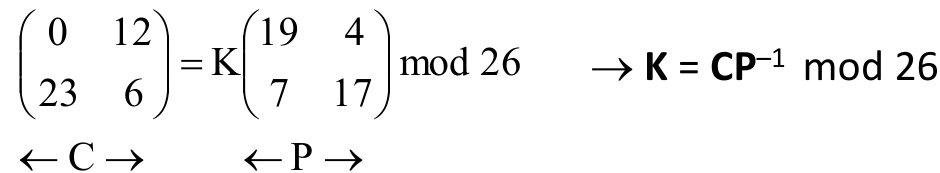
\includegraphics[width=102.90mm,height=47.52mm]{../../images/llm/page_107_img_01.png}%
\end{textblock*}

\end{document}
